\documentclass{article}

\usepackage{fancyhdr}
\usepackage{extramarks}
\usepackage{amsmath}
\usepackage{amsthm}
\usepackage{amsfonts}
\usepackage{tikz}
\usepackage[plain]{algorithm}
\usepackage{algpseudocode}
\usepackage{xcolor}
\usepackage{enumitem}
\usepackage{amssymb}
\usepackage{todonotes}
\usepackage{mathtools}
\usepackage{wasysym}
\usepackage{cancel}
\usepackage{phaistos}

\usetikzlibrary{automata,positioning}

%
% Basic Document Settings
%

\topmargin=-0.45in
\evensidemargin=0in
\oddsidemargin=0in
\textwidth=6.5in
\textheight=9.0in
\headsep=0.25in

\linespread{1.1}

\pagestyle{fancy}
\lhead{\hmwkAuthorName}
\chead{\hspace{2.5cm} \hmwkClass\ (\hmwkClassInstructor): \hmwkTitle}
\rhead{\firstxmark}
\lfoot{\lastxmark}
\cfoot{\thepage}

\renewcommand\headrulewidth{0.4pt}
\renewcommand\footrulewidth{0.4pt}

\setlength\parindent{0pt}

%
% Create Problem Sections
%

\newcommand{\enterProblemHeader}[1]{
    \nobreak\extramarks{}{Problem \arabic{#1} continued on next page\ldots}\nobreak{}
    \nobreak\extramarks{Problem \arabic{#1} (continued)}{Problem \arabic{#1} continued on next page\ldots}\nobreak{}
}

\newcommand{\exitProblemHeader}[1]{
    \nobreak\extramarks{Problem \arabic{#1}}{Problem \arabic{#1} continued on next page\ldots}\nobreak{}
    \stepcounter{#1}
    \nobreak\extramarks{Problem \arabic{#1}}{}\nobreak{}
}

\newcount\colveccount
\newcommand*\colvec[1]{
        \global\colveccount#1
        \begin{pmatrix}
        \colvecnext
}
\def\colvecnext#1{
        #1
        \global\advance\colveccount-1
        \ifnum\colveccount>0
                \\
                \expandafter\colvecnext
        \else
                \end{pmatrix}
        \fi
}

\setcounter{secnumdepth}{0}
\newcounter{partCounter}
\newcounter{homeworkProblemCounter}
\setcounter{homeworkProblemCounter}{1}
\nobreak\extramarks{Problem \arabic{homeworkProblemCounter}}{}\nobreak{}

%
% Homework Problem Environment
%
% This environment takes an optional argument. When given, it will adjust the
% problem counter. This is useful for when the problems given for your
% assignment aren't sequential. See the last 3 problems of this template for an
% example.
%
\newenvironment{homeworkProblem}[1][-1]{
    \ifnum#1>0
        \setcounter{homeworkProblemCounter}{#1}
    \fi
    \section{Problem \arabic{homeworkProblemCounter}}
    \setcounter{partCounter}{1}
    \enterProblemHeader{homeworkProblemCounter}
}{
    \exitProblemHeader{homeworkProblemCounter}
}

%
% Homework Details
%   - Title
%   - Due date
%   - Class
%   - Section/Time
%   - Instructor
%   - Author
%

\newcommand{\hmwkTitle}{Assignment 2}
\newcommand{\hmwkDueDate}{September 28, 2018}
\newcommand{\hmwkClass}{Probability \& Statistics}
\newcommand{\hmwkClassTime}{Spring Semester}
\newcommand{\hmwkClassInstructor}{Prof. D. Eynard}
\newcommand{\hmwkAuthorName}{\textbf{A. Romanelli} / \textbf{A. Vicini}}

%
% Title Page
%

\title{
    \vspace{2in}
    \textmd{\textbf{\hmwkClass:\ \hmwkTitle}}\\
    \normalsize\vspace{0.1in}\small{Due\ on\ \hmwkDueDate\ at 8:30am}\\
    \vspace{0.1in}\large{\textit{\hmwkClassInstructor}}
    \vspace{3in}
}

\author{\hmwkAuthorName}
\date{}

\renewcommand{\part}[1]{\textbf{\large Part \Alph{partCounter}}\stepcounter{partCounter}\\}

%
% Various Helper Commands
%

% Useful for algorithms
\newcommand{\alg}[1]{\textsc{\bfseries \footnotesize #1}}

% For derivatives
\newcommand{\deriv}[1]{\frac{\mathrm{d}}{\mathrm{d}x} (#1)}

% For partial derivatives
\newcommand{\pderiv}[2]{\frac{\partial}{\partial #1} (#2)}

% Integral dx
\newcommand{\dx}{\mathrm{d}x}

% Alias for the Solution section header
\newcommand{\solution}{\textbf{\large Solution}}

% Probability commands: Expectation, Variance, Covariance, Bias
\newcommand{\E}{\mathrm{E}}
\newcommand{\Var}{\mathrm{Var}}
\newcommand{\Cov}{\mathrm{Cov}}
\newcommand{\Bias}{\mathrm{Bias}}

\begin{document}

\maketitle

\pagebreak

\begin{homeworkProblem}
	\begin{enumerate}[label=\textbf{\alph*)}]
		\item The proof that $\Omega$ is a discrete probability space lies within the definition of the set $\Omega$ itself which is given to us being the set of all integer numbers between 1 and 12, thus a bounded interval and surely a finite one.
		\item In order to prove that $p$ is a probability measure we need to show the three following properties:
		\begin{enumerate}[label=\roman*.]
			\item Normalisation
			\item Positivity
			\item Additivity for disjoint sets
		\end{enumerate}
		\paragraph{i. Normalisation} We want to show that $P(\Omega) = 1$, knowing that $P(\{\omega\}) = \frac1{12}, \forall \omega \in \Omega$, as given to us by the problem's premises. This is indeed true if we compute the summation of the probabilities of all the faces of the given die:
		$$\sum_{i = 1}^{12} \left(\frac1{12}\right) = \frac1{12} + \frac1{12} + \dots + \frac1{12} = 1$$ 
		\paragraph{ii. Positivity} To prove this property, we will need to make sure that it doesn't exist a $P(\{\omega\}) < 0, \forall \omega \in \Omega$. But as we already know that all the faces of the die share the same probability $P(\{\omega\}) = \frac1{12} > 0$, thus $P(\{\omega\}) > 0, \forall \omega \in \Omega$.
		\paragraph{iii. Additivity} Let's consider to possible events of $\Omega$, namely $A$ and $B$. When throwing the die, the chance of an event $\omega \in (A \cup B)$ happening is twice the chance of an event $\omega \in A$ or $\omega \in B$, which we know being $\frac1{12}$.
		$$P(A \cup B) = P(A) + P(B)$$
		$$\sum_{\omega \in A \cup B} p(\omega) = \sum_{\omega \in A} p(\omega) + \sum_{\omega \in B}p(\omega)$$
		$$\frac2{12} = \frac1{12} + \frac1{12}$$
		$$\frac2{12} = \frac2{12} \qed$$
		Moreover we can say that over a single throw there can be no overlapping of events, which means that all events are disjoint sets.
		\item Given the following set of events:
		\begin{itemize}
			\item $A_1:$ the outcome is a even number : $\{2,4,6,8,10,12\}$
			\item $A_2:$ the outcome is greater than six : $\{7,8,9,10,11,12\}$
			\item $A_3:$ the outcome is a number which is a multiple of three : $\{3,6,9,12\}$
		\end{itemize}
		We can see already that we cannot compute $P(\bigcup_{i=1}^3 A_i)$ because there are clearly elements in common between the three events, like the outcome involving a 12, which is contained within each of the three events. Thus, we cannot compute the probability because $\exists i, j \in \{1,2,3\} : A_i \cap A_j \neq \emptyset$.
		\item For the inclusion/exclusion principle, we have no constraints and we can thus compute the probability of $P(A_1 \cup A_2 \cup A_3)$:
		$$P(A_1) + P(A_2) + P(A_3) - P(A_1 \cap A_2) - P(A_2 \cap A_3) - P(A_3 \cap A_1) + P(A_1 \cap A_2 \cap A_3)$$
		$$\frac{|A_1|}{12} + \frac{|A_2|}{12} + \frac{|A_3|}{12} - \frac{|A_1 \cap A_2|}{12} - \frac{|A_2 \cap A_3|}{12} - \frac{|A_3 \cap A_1|}{12} + \frac{|A_1 \cap A_2 \cap A_3|}{12}$$
		$$\frac12 + \frac12 + \frac13 - \frac14 - \frac16 - \frac16 + \frac1{12} = 0.8\overline{3}$$
	\end{enumerate}
\end{homeworkProblem}
\begin{homeworkProblem}
	\begin{enumerate}[label=\textbf{\alph*)}]
		\item Based on my catch our estimate would be to have a 30\% of red fishes and 70\% of white fishes, although according to the \emph{Law of Large Numbers} we would need several attempts to verify whether this estimate is accurate or not.
		\item $$p(\text{catch}) = \frac{90 \times 89 \times 88 \times 87 \times 86 \times 85 \times 84 \times 10 \times 9 \times 8}{100 \times 99 \times 98 \times 97 \times 96 \times 95 \times 94 \times 93 \times 92 \times 91} \approx 0.000431...$$ This gives us the probability of one of the multiple permutations of our catch. In order to compute all these possible permutation we need to compute them with the following formula: 
		$$\frac{10!}{7! \cdot 3!} = 120$$
		$$p(\text{catch}) \times 120 \approx 0.05179$$
		\item $$p(\text{catch}) = \frac{10 \times 9 \times 8 \times 7 \times 6 \times 5 \times 4 \times 90 \times 89 \times 88}{100 \times 99 \times 98 \times 97 \times 96 \times 95 \times 94 \times 93 \times 92 \times 91} \approx 6.786 \times 10^{-9}$$ Again, we need to multiply this by the number of possible permutations, which are still 120:
		$$ 6.786 \times 10^{-9} \times 120 = 8.144 \times 10^{-7}$$
		\item $0\%$, since we couldn't possibly catch 7 white fishes if there are only five in the pond.
		\item $$\frac{R! \cdot (N-R)! \cdot (N - n)!}{N! \cdot (R -r)! \cdot (W -w)!} \cdot \frac{n!}{r!\cdot w!}$$
	\end{enumerate}
\end{homeworkProblem}
\begin{homeworkProblem}
	This strategy is not really a viable one if what we aim for is to have a higher percentage of male against females and here's why: \\\\
	Let's take $2^n$ of the female population as a sample:
	\begin{center}
		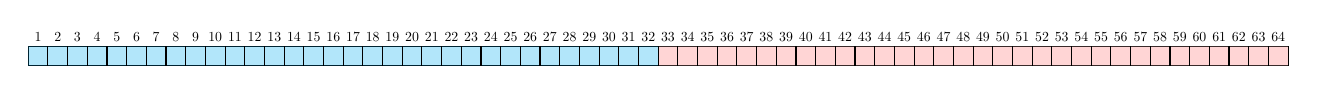
\begin{tikzpicture}[scale=0.25]
			\draw (0,0) -- (64, 0) -- (64,1) -- (0,1) -- cycle;
			\draw[fill=cyan, opacity=0.3] (0,0) rectangle (32,1);
			\draw[fill=pink, opacity=0.66] (32,0) rectangle (64,1);
			\foreach \i in {1, ..., 63} {
				\draw (\i,0) -- (\i, 1);
				\node[above, scale=0.5] at (\i-0.5,1) {\i};
			};
			\node[above, scale=0.5] at (64-0.5,1) {64};
		\end{tikzpicture}
	\end{center}
	Under the assumption that we have equal birth rate between males and females, half of those women are going to give birth to a {\color{purple}girl}, whereas the other half is going to give birth to a {\color{cyan}boy}. \\ \\
	Now, only the women who did give birth to a male are going to give birth again:
	\begin{center}
		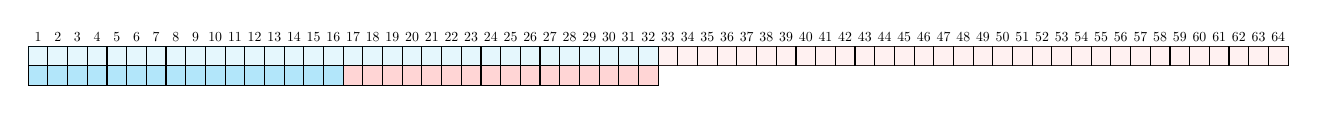
\begin{tikzpicture}[scale=0.25]
			\draw (0,0) -- (64, 0) -- (64,1) -- (0,1) -- cycle;
			\draw[fill=cyan, opacity=0.1] (0,0) rectangle (32,1);
			\draw[fill=pink, opacity=0.22] (32,0) rectangle (64,1);
			\foreach \i in {1, ..., 63} {
				\draw (\i,0) -- (\i, 1);
				\node[above, scale=0.5] at (\i-0.5,1) {\i};
			};
			\node[above, scale=0.5] at (64-0.5,1) {64};
			\draw[fill=cyan, opacity=0.3] (0,0) rectangle (16,-1);
			\draw[fill=pink, opacity=0.66] (16,0) rectangle (32,-1);
			\draw (0,0) -- (32, 0) -- (32,-1) -- (0,-1) -- cycle;
			\foreach \i in {1, ..., 31} {
				\draw (\i,0) -- (\i, -1);
			}
		\end{tikzpicture}
	\end{center}
	To better visualise what's going on, we're going to shift the sample so that we always have the midpoint in the middle of the page, since at each iteration we lose half of the population which gave birth to a girl.
	We repeat this until there's no one else left who can give birth to anyone.
	\begin{center}
		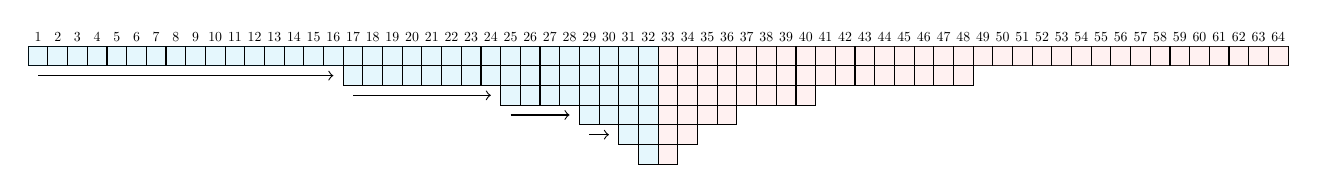
\begin{tikzpicture}[scale=0.25]
			\draw (0,0) -- (64, 0) -- (64,1) -- (0,1) -- cycle;
			\draw[fill=cyan, opacity=0.1] (0,0) rectangle (32,1);
			\draw[fill=pink, opacity=0.22] (32,0) rectangle (64,1);
			\foreach \i in {1, ..., 63} {
				\draw (\i,0) -- (\i, 1);
				\node[above, scale=0.5] at (\i-0.5,1) {\i};
			};
			\node[above, scale=0.5] at (64-0.5,1) {64};
			\draw[->] (0.5,-0.5) -- (15.5, -0.5);
			
			\draw[fill=cyan, opacity=0.1] (0+16,0) rectangle (16+16,-1);
			\draw[fill=pink, opacity=0.22] (16+16,0) rectangle (32+16,-1);
			\draw (0+16,0) -- (32+16, 0) -- (32+16,-1) -- (0+16,-1) -- cycle;
			\foreach \i in {1, ..., 31} {
				\draw (\i+16,0) -- (\i+16, -1);
			}
			\draw[->] (16.5,-1.5) -- (23.5, -1.5);
			
			\draw[fill=cyan, opacity=0.1] (0+24,-1) rectangle (16+16,-2);
			\draw[fill=pink, opacity=0.22] (16+16,-1) rectangle (32+8,-2);
			\draw (0+24,-1) -- (0+24,-2) -- (16+24,-2) -- (16+24,-1) -- cycle;
			\foreach \i in {1, ..., 16} {
				\draw (\i+24,-1) -- (\i+24, -2);
			}
			\draw[->] (24.5,-2.5) -- (27.5, -2.5);

			
			\draw[fill=cyan, opacity=0.1] (0+28,-2) rectangle (16+16,-3);
			\draw[fill=pink, opacity=0.22] (16+16,-2) rectangle (32+4,-3);
			\draw (0+28, -2) -- (0+28,-3) -- (16+20,-3) -- (16+20,-2) -- cycle;
			\foreach \i in {1, ..., 8} {
				\draw (\i+28,-2) -- (\i+28, -3);
			}	
			\draw[->] (28.5,-3.5) -- (29.5, -3.5);

			
						
			\draw[fill=cyan, opacity=0.1] (0+30,-3) rectangle (16+16,-4);
			\draw[fill=pink, opacity=0.22] (16+16,-3) rectangle (32+2,-4);
			\draw (0+30, -3) -- (0+30,-4) -- (16+18,-4) -- (16+18,-3) -- cycle;
			\foreach \i in {1, ..., 4} {
				\draw (\i+30,-3) -- (\i+30, -4);
			}				
									
			\draw[fill=cyan, opacity=0.1] (0+31,-4) rectangle (16+16,-5);
			\draw[fill=pink, opacity=0.22] (16+16,-4) rectangle (32+1,-5);
			\draw (0+31, -4) -- (0+31,-5) -- (16+17,-5) -- (16+17,-4) -- cycle;
			\foreach \i in {1, ..., 2} {
				\draw (\i+31,-4) -- (\i+31, -5);
			}			
		\end{tikzpicture}
	\end{center}
	It's clearly a zero-sum process. Whenever a girl is born, a male must also be born and the two cancel out, not influencing the ratio between females and males. \\ \\
	For any $n$ of women, if we let the boys being born as $B$ and the girls as $G$ we know that $B = G =\frac n2$ we can say that there's going to be $\log_2 (n)$ generations before no one can give birth. \\ \\
	If every woman is going to stop as soon as she gives birth to a woman, then we can certainly say that the number of girls is going to be surely $n$. We can compute the number of boys $B$ as the following summation:
	$$\sum_{i=1}^{\log_2n}\left(\frac1{2^i}n\right)$$
	But this can really be simplified to: 
	$$\sum_{i=1}^{\log_2n}\left(\frac1{2^i}n\right) = n -1$$
	Which clearly shows how $B < G, \forall n \in \mathbb{N}$ and thus this is not a viable to way to increase the percentage of males in the realm.
\end{homeworkProblem}
\begin{homeworkProblem}
	To tackle this problem we can try to think about it in smaller terms and see how this does scale and if the scale of the problem (aka the seats available) count towards the solution.
	Let's imagine we have only two seats:
	\begin{center}
		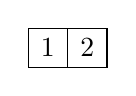
\begin{tikzpicture}[scale=0.5]
			\draw (0,0) -- (2,0) -- (2,1) -- (0,1) -- cycle;
			\draw (1,0) -- (1,1);
			\node at (0.5, 0.5) {1};
			\node at (1.5, 0.5) {2};
		\end{tikzpicture}
	\end{center}
	The chances of the first person getting his seat is exactly $\frac12$, to randomly get his rightful place or get the wrong one. 
	If we scale this problem up to 3 seats we get the following:
	\begin{center}
		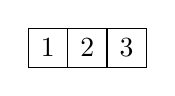
\begin{tikzpicture}[scale=0.5]
			\draw (0,0) -- (3,0) -- (3,1) -- (0,1) -- cycle;
			\draw (1,0) -- (1,1);
			\draw (2,0) -- (2,1);
			\node at (0.5, 0.5) {1};
			\node at (1.5, 0.5) {2};
			\node at (2.5, 0.5) {3};
		\end{tikzpicture}
	\end{center}
	Where in $\frac13$ of the cases, the person who lost the ticker finds again the right place, whereas in the other cases it's taking someone else's spot. \\
	If it is taking someone else's spot $\frac23$ of the cases, we need to count what's the chance that out of the two seats left the second guy picks the seat of the first guy, bringing back balance into the situation and granting the third person the rightful seat. \\
	But that was the exact same situation that we explored previously, where with two seats we would have a 50\% chance! We can then start to explore a recursive way to model this problem. \\ \\
	Let's reconsider again the problem but with the 100 seats:
	\begin{center}
		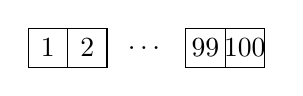
\begin{tikzpicture}[scale=0.5]
			\draw (0,0) -- (2,0) -- (2,1) -- (0,1) -- cycle;
			\draw (1,0) -- (1,1);
			\node at (3,0.5) {\dots};
			\draw (4,0) -- (6,0) -- (6,1) -- (4,1) -- cycle;
			\draw (5,0) -- (5,1);
			\node at (0.5, 0.5) {1};
			\node at (1.5, 0.5) {2};
			\node at (4.5, 0.5) {99};
			\node at (5.5, 0.5) {100};
		\end{tikzpicture}
	\end{center}
	In this instance we will proceed exactly as we did for the previous example.
	The first person boarding the plane has a $\frac1{100}$ of getting the right spot but then we need to add to this chance the possibility of him sitting somewhere else and stealing a seat. \\ 
	This happens in the rest of the cases and we need to consider what's the chance of \underline{NOT} getting the seat of the last person, hence $\frac{99}{100} - \frac1{100} = \frac{98}{100}$ and we need to multiply this by the probability of the subproblem for 99 seats.
	We can then come up with the following formula:
	$$p(n) = \frac1n + \frac{n-2}n\cdot p(n-1)$$
	With $n \geq 2$ and $p(2) = \frac12$ \\
	$$p(3) = \frac13 + \frac13 \cdot \frac12 = \frac13 + \frac16 = \frac12$$
	$$p(4) = \frac14 + \frac24 \cdot \frac12 = \frac14 + \frac14 = \frac12 $$
	We can see that there is a steady trend, can we prove though that $p(n) = \frac12, \forall n \in \mathbb{N}$? \\ \\
	We'll give it a shot by induction: \\
	We set our base case and verify whether $p(2) = \frac12$
	$$\frac12 + \frac{2-2}2 \cdot p(1) = \frac12$$
	$$\frac12 + 0 = \frac12$$
	Our formula holds for $n = 2$, let's now assume that $p(n) = \frac12$ is true for some $n$ and attempt to prove this for $n+1$.
	$$\frac1{n+1} + \frac{n+1-2}{n+1}\cdot p(n) = \frac12$$
	$$\frac1{n+1} + \frac{n+1-2}{n+1}\cdot \frac12 = \frac12$$
	$$\frac2{n+1} + \frac{n+1-2}{n+1} = 1$$
	$$\frac2{n+1} + \frac{n-1}{n+1} = 1$$
	$$\frac{n+1}{n+1} = 1 \Rightarrow 1 = 1, \forall n \in \mathbb{N}$$
\end{homeworkProblem}
\end{document}
